\documentclass[11pt]{article}
\usepackage[letterpaper,margin=0.9in]{geometry}
\usepackage{amsmath,amssymb}
\usepackage{graphicx}
\usepackage[T1]{fontenc}
\usepackage{lmodern}
\usepackage{microtype}
\setlength{\parindent}{0pt}
\setlength{\parskip}{0.45em}
\newcommand{\KL}{\operatorname{KL}}

\title{NLP Assignment 1: Solutions}
\author{PAN CHANGXUN\\Student ID: 2024011323}
\date{August 2026}

\begin{document}
\maketitle
\vspace{-2em}

\section*{Problem 1: CFG}
\subsection*{1. Chomsky Normal Form}

There are no $\epsilon$-productions.  Eliminate the unit productions
\[
\mathrm{NP}\to\mathrm{PropN},\quad
\mathrm{Nom}\to\mathrm{Noun},\quad
\mathrm{VP}\to\mathrm{Verb}
\]
by copying their terminal rules, then remove the unreachable $\mathrm{PropN}$.
An equivalent CNF grammar is
\[
\begin{array}{rcl}
S&\to&\mathrm{NP}\ \mathrm{VP},\\
\mathrm{NP}&\to&\mathrm{Det}\ \mathrm{Nom}\mid\texttt{Houston},\\
\mathrm{Nom}&\to&\mathrm{Noun}\ \mathrm{Nom}\mid\texttt{book}\mid\texttt{flight},\\
\mathrm{VP}&\to&\mathrm{Verb}\ \mathrm{NP}\mid\texttt{booked},\\
\mathrm{Det}&\to&\texttt{the}\mid\texttt{a},\\
\mathrm{Noun}&\to&\texttt{book}\mid\texttt{flight},\\
\mathrm{Verb}&\to&\texttt{booked}.
\end{array}
\]
Every rule is now of the form $A\to BC$ or $A\to a$.

\subsection*{2. CKY for ``the book booked''}

For $w_1=\texttt{the}$, $w_2=\texttt{book}$, and
$w_3=\texttt{booked}$, the completed chart is
\[
\begin{array}{c|ccc}
&j=1&j=2&j=3\\ \hline
i=1&\{\mathrm{Det}\}&\{\mathrm{NP}\}&\{S\}\\
i=2&&\{\mathrm{Noun},\mathrm{Nom}\}&\varnothing\\
i=3&&&\{\mathrm{Verb},\mathrm{VP}\}
\end{array}
\]
$C_{1,2}$ contains $\mathrm{NP}$ because
$\mathrm{NP}\to\mathrm{Det}\ \mathrm{Nom}$, and $C_{1,3}$ contains $S$
because $S\to\mathrm{NP}\ \mathrm{VP}$.  Thus $S\in C_{1,3}$ and the
sentence is \textbf{accepted}.

\newpage
\section*{Problem 2: Bigram Model}
\subsection*{1. Add-one smoothing}

The vocabulary is
\[
\{\texttt{<s>},\texttt{I},\texttt{am},\texttt{Sam},\texttt{</s>},
\texttt{do},\texttt{not},\texttt{like},\texttt{green},\texttt{eggs},
\texttt{and}\},
\]
so $|V|=11$.  Since $C(\texttt{am})=3$ and
$C(\texttt{am Sam})=2$,
\[
P(\texttt{Sam}\mid\texttt{am})
=\frac{2+1}{3+11}
=\boxed{\frac{3}{14}\approx0.2143}.
\]

\subsection*{2. Model without an end symbol}

The unsmoothed estimates are
\[
P(\texttt{a}\mid\texttt{<s>})=P(\texttt{b}\mid\texttt{<s>})
=P(\texttt{a}\mid\texttt{a})=P(\texttt{b}\mid\texttt{a})
=P(\texttt{a}\mid\texttt{b})=P(\texttt{b}\mid\texttt{b})=\frac12.
\]
Each two-word string has probability $(1/2)^2=1/4$, so
\[
\sum_{w_1,w_2\in\{\texttt{a},\texttt{b}\}}P(w_1w_2)
=4\cdot\frac14=\boxed{1}.
\]
Each three-word string has probability $(1/2)^3=1/8$, so
\[
\sum_{w_1,w_2,w_3\in\{\texttt{a},\texttt{b}\}}P(w_1w_2w_3)
=8\cdot\frac18=\boxed{1}.
\]
Thus every fixed length receives total mass $1$; over all lengths the mass is
$\sum_{n\ge1}1=\infty$.  Without a stopping symbol, this is not a probability
distribution over finite sentences.

\newpage
\section*{Problem 3: RLHF}
\subsection*{1. Optimal policy}

Fix $x$, and let $q(y)=\pi_{\mathrm{ref}}(y\mid x)$ and
$r_y=r(x,y)$.  Define
\[
Z(x)=\sum_{y'}q(y')e^{r_{y'}/\beta},\qquad
\pi^*(y\mid x)=\frac{q(y)e^{r_y/\beta}}{Z(x)}.
\]
For any $\pi$,
\begin{align*}
\KL(\pi\|\pi^*)
&=\KL(\pi\|q)-\frac1\beta\sum_y\pi(y\mid x)r_y+\log Z(x),
\end{align*}
so the per-prompt objective satisfies
\[
\sum_y\pi(y\mid x)r_y-\beta\KL(\pi\|q)
=\beta\log Z(x)-\beta\KL(\pi\|\pi^*).
\]
Since KL divergence is nonnegative, the maximum is attained at
$\pi=\pi^*$.  The unrestricted full objective separates over prompts, so this
holds for every $x$, proving Eq.~(3)--(4).

\subsection*{2. Direct calculation}

No. Computing $Z(x)$ requires summing over all possible response sequences and
evaluating their rewards, which is computationally intractable. \emph{(20 words)}

\subsection*{3. Deriving Eq.~(7)}

Rearranging Eq.~(3) gives
\[
r(x,y)=\beta\log\frac{\pi^*(y\mid x)}
{\pi_{\mathrm{ref}}(y\mid x)}+\beta\log Z(x).
\]
Set $\pi^*=\pi_\theta$.  For responses paired under the same prompt, the
$\beta\log Z(x)$ terms cancel:
\[
r(x,y_w)-r(x,y_l)
=\beta\log\frac{\pi_\theta(y_w\mid x)}{\pi_{\mathrm{ref}}(y_w\mid x)}
-\beta\log\frac{\pi_\theta(y_l\mid x)}{\pi_{\mathrm{ref}}(y_l\mid x)}.
\]
Substitution into Eq.~(6) yields
\[
\mathcal L_\pi(\theta)=-\frac1N\sum_{i=1}^N\log\sigma\!\left(
\beta\log\frac{\pi_\theta(y_w^{(i)}\mid x^{(i)})}
{\pi_{\mathrm{ref}}(y_w^{(i)}\mid x^{(i)})}
-\beta\log\frac{\pi_\theta(y_l^{(i)}\mid x^{(i)})}
{\pi_{\mathrm{ref}}(y_l^{(i)}\mid x^{(i)})}
\right),
\]
which is Eq.~(7).

\newpage
\section*{Problem 4B: Code Completion}

I completed all four TODOs in \texttt{problem\_word2vec/word2vec.py}: the two
embedding layers, the negative-sampling loss, frequency-based negative
sampling, and the training loop.  The completed source file is submitted
separately as required.

\section*{Problem 4C: Unity 6 Tutorial}
\subsection*{1. What I learned}

The most interesting part of the tutorial was seeing how Unity combines
transforms, colliders, rigid-body physics, and materials.  I built ramps and
stairs from simple cubes, and the robot interacted with them through gravity
and collision instead of passing through the geometry.  I also learned that
materials tile across resized objects, which makes rapid prototyping easier.
The tutorial further showed how lighting, post-processing, VFX, collectibles,
UI, and animation can turn a basic blockout into a playable scene.

\begin{figure}[htbp]
    \centering
    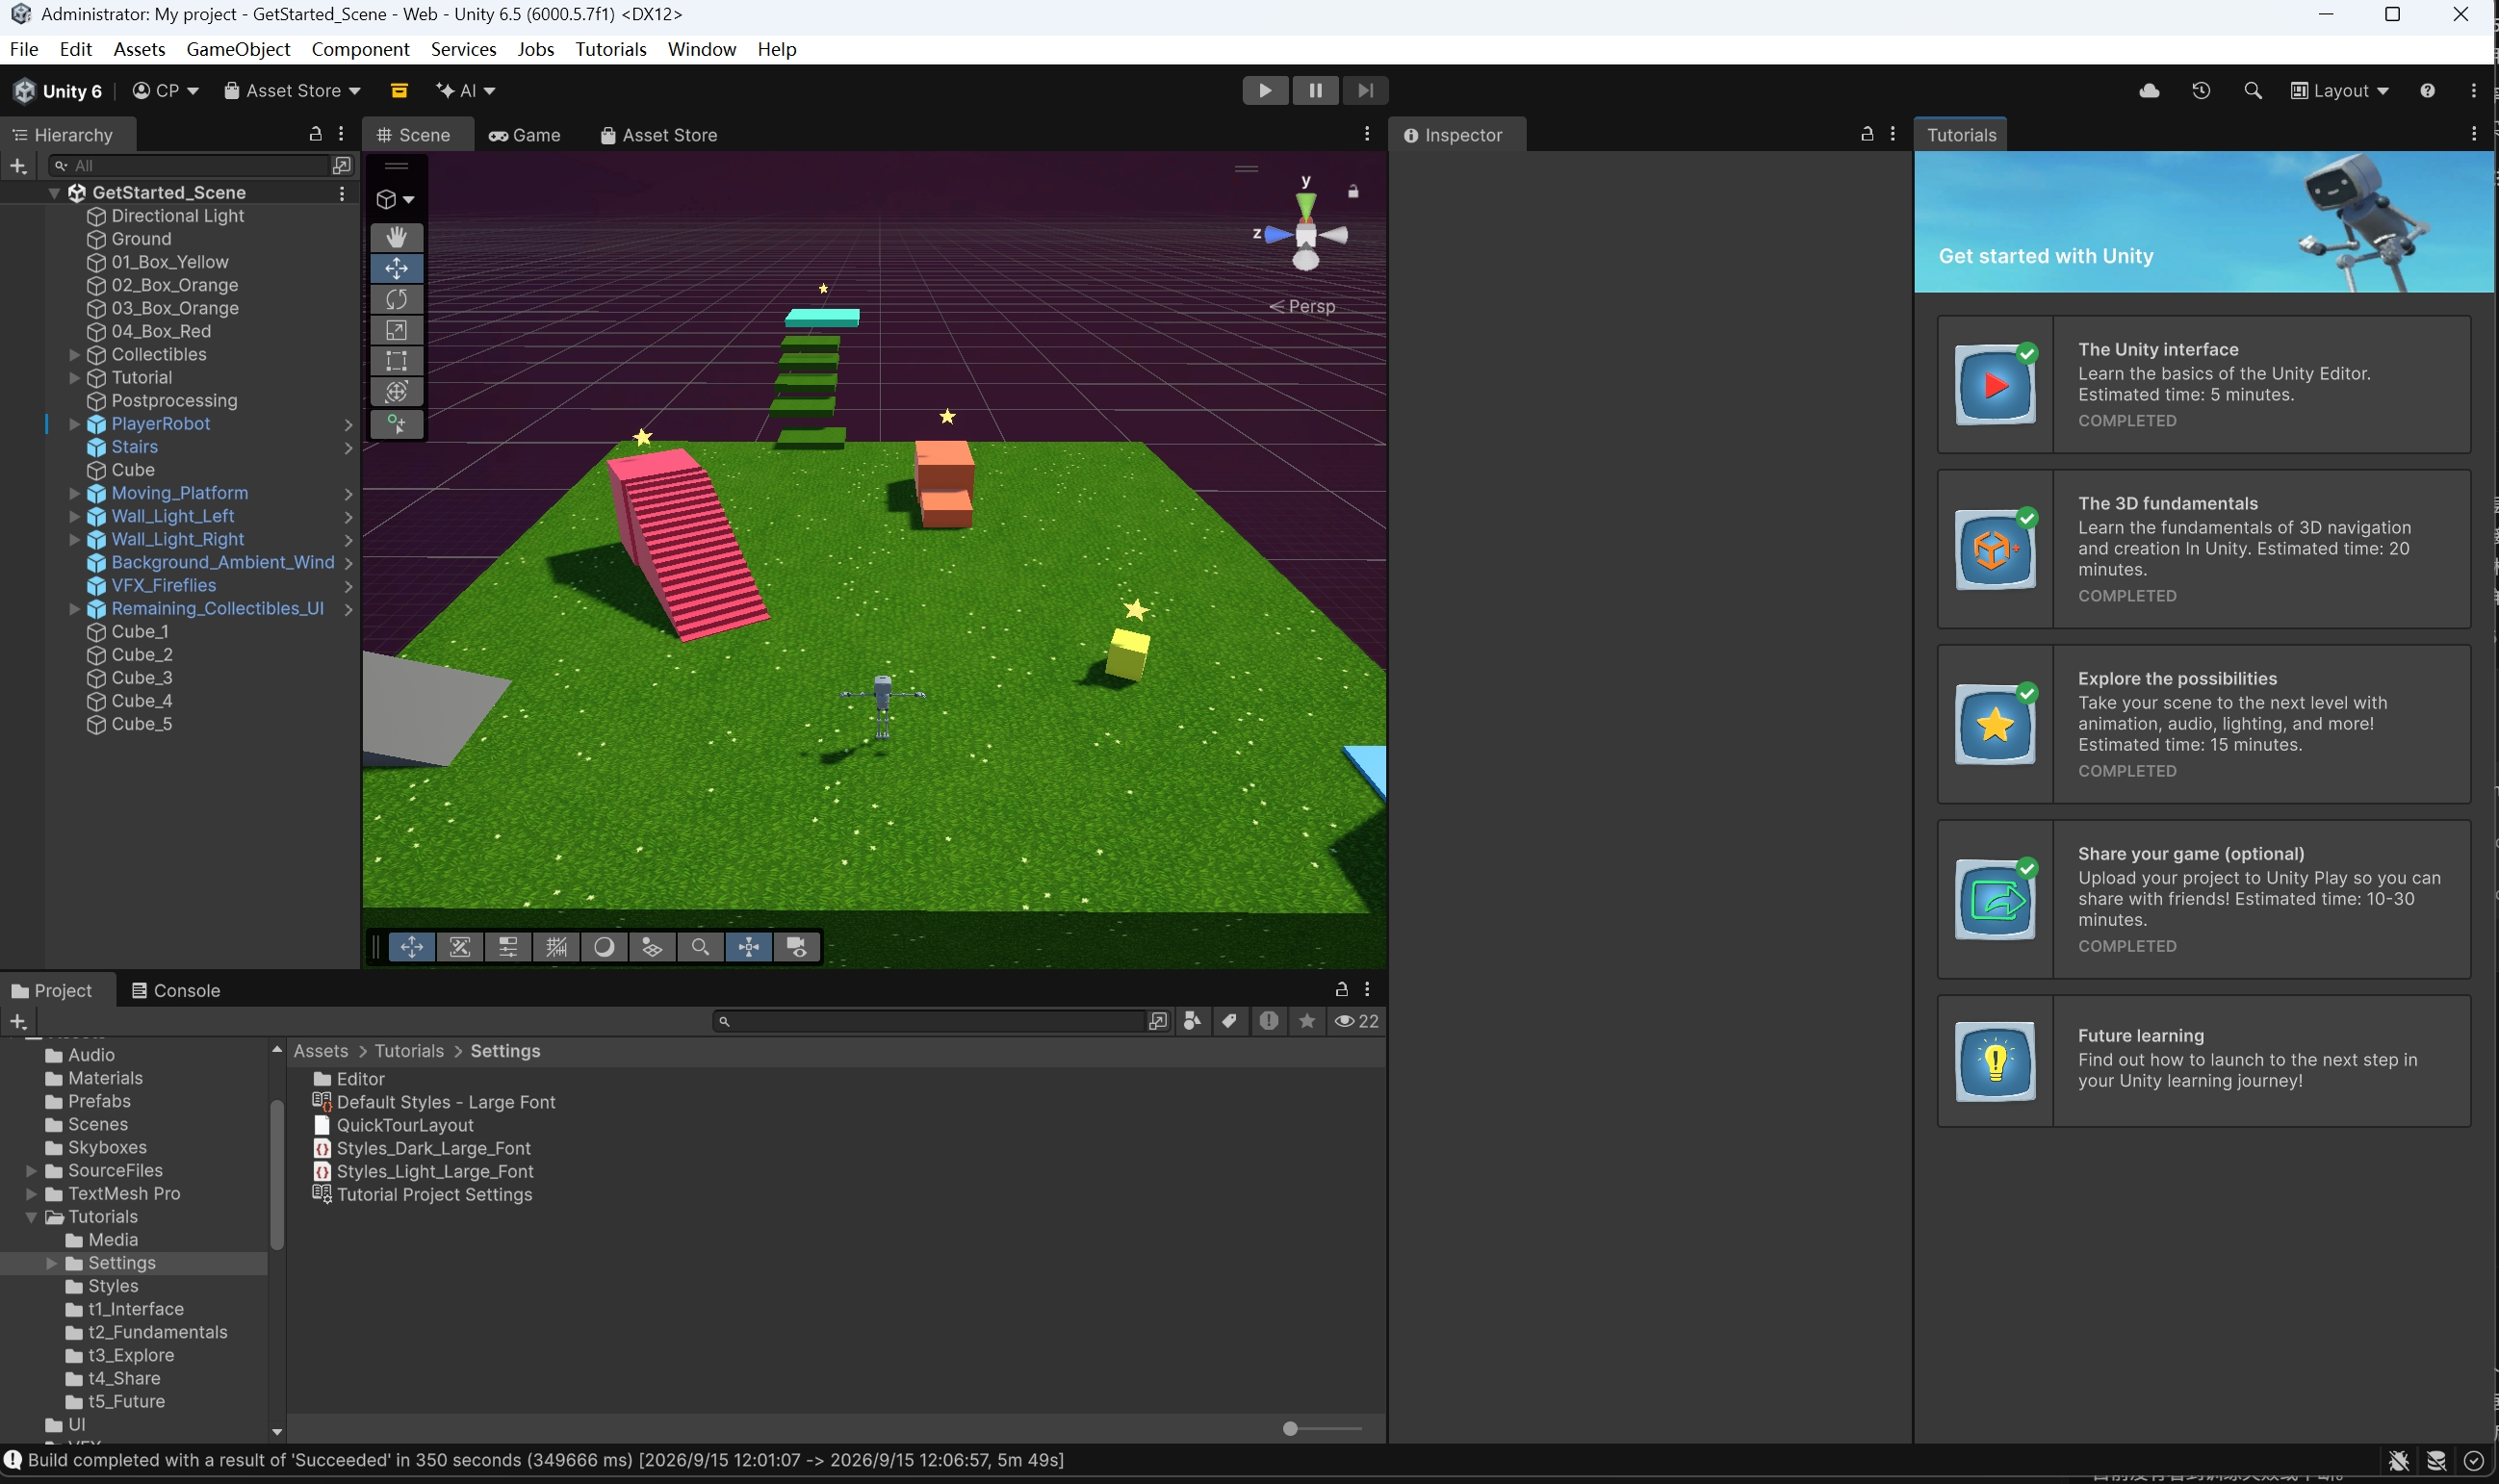
\includegraphics[width=0.94\textwidth]{final.jpg}
    \caption{The final robot scene after completing the required tutorial sections.}
\end{figure}

\subsection*{2. Scene extension}

I expanded the play area to $66\times74$ units and surrounded it with
grass-topped collision walls so the robot stays inside the scene.  I added
more routes to the collectibles, including ramps, stairs, and elevated
platforms.  I also laid out paths, planted trees and flower beds, and adjusted
the lighting, sky, and visual effects to make the level feel more like a small
park.

\begin{figure}[htbp]
    \centering
    \begin{minipage}[t]{0.49\textwidth}
        \centering
        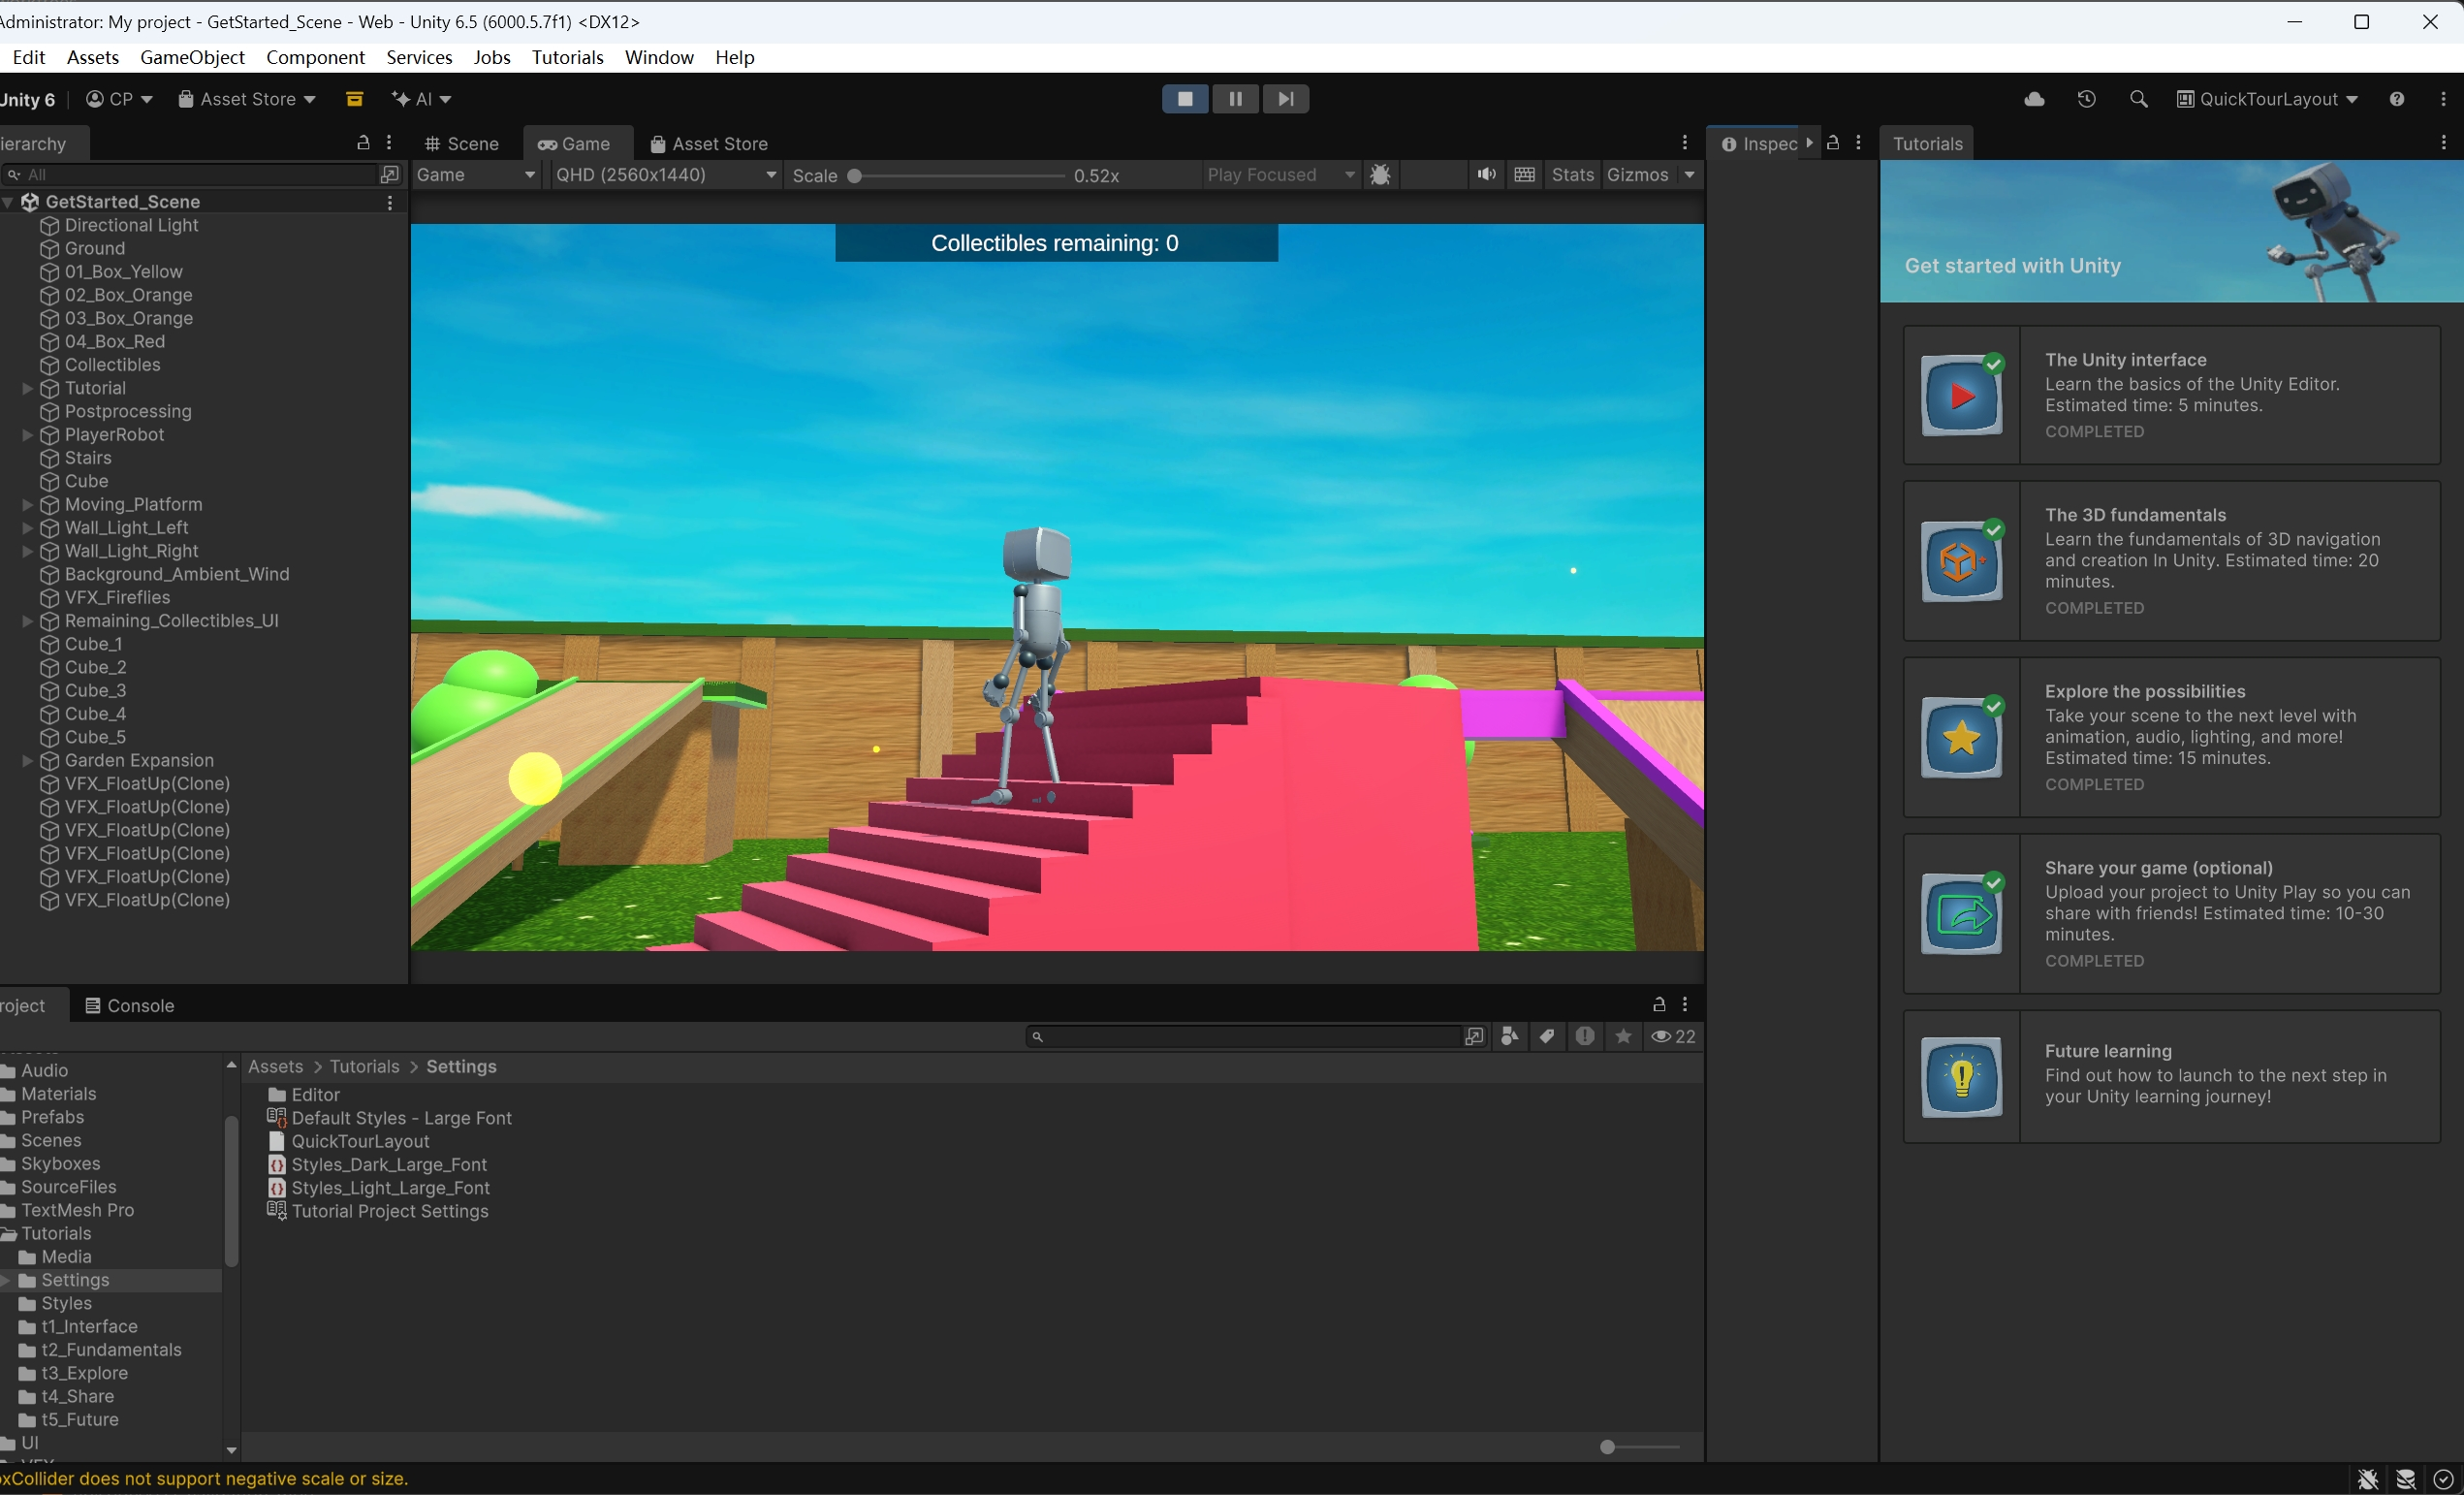
\includegraphics[width=\linewidth]{u6.jpg}
        \small (a) Stair route and enclosed play area
    \end{minipage}\hfill
    \begin{minipage}[t]{0.49\textwidth}
        \centering
        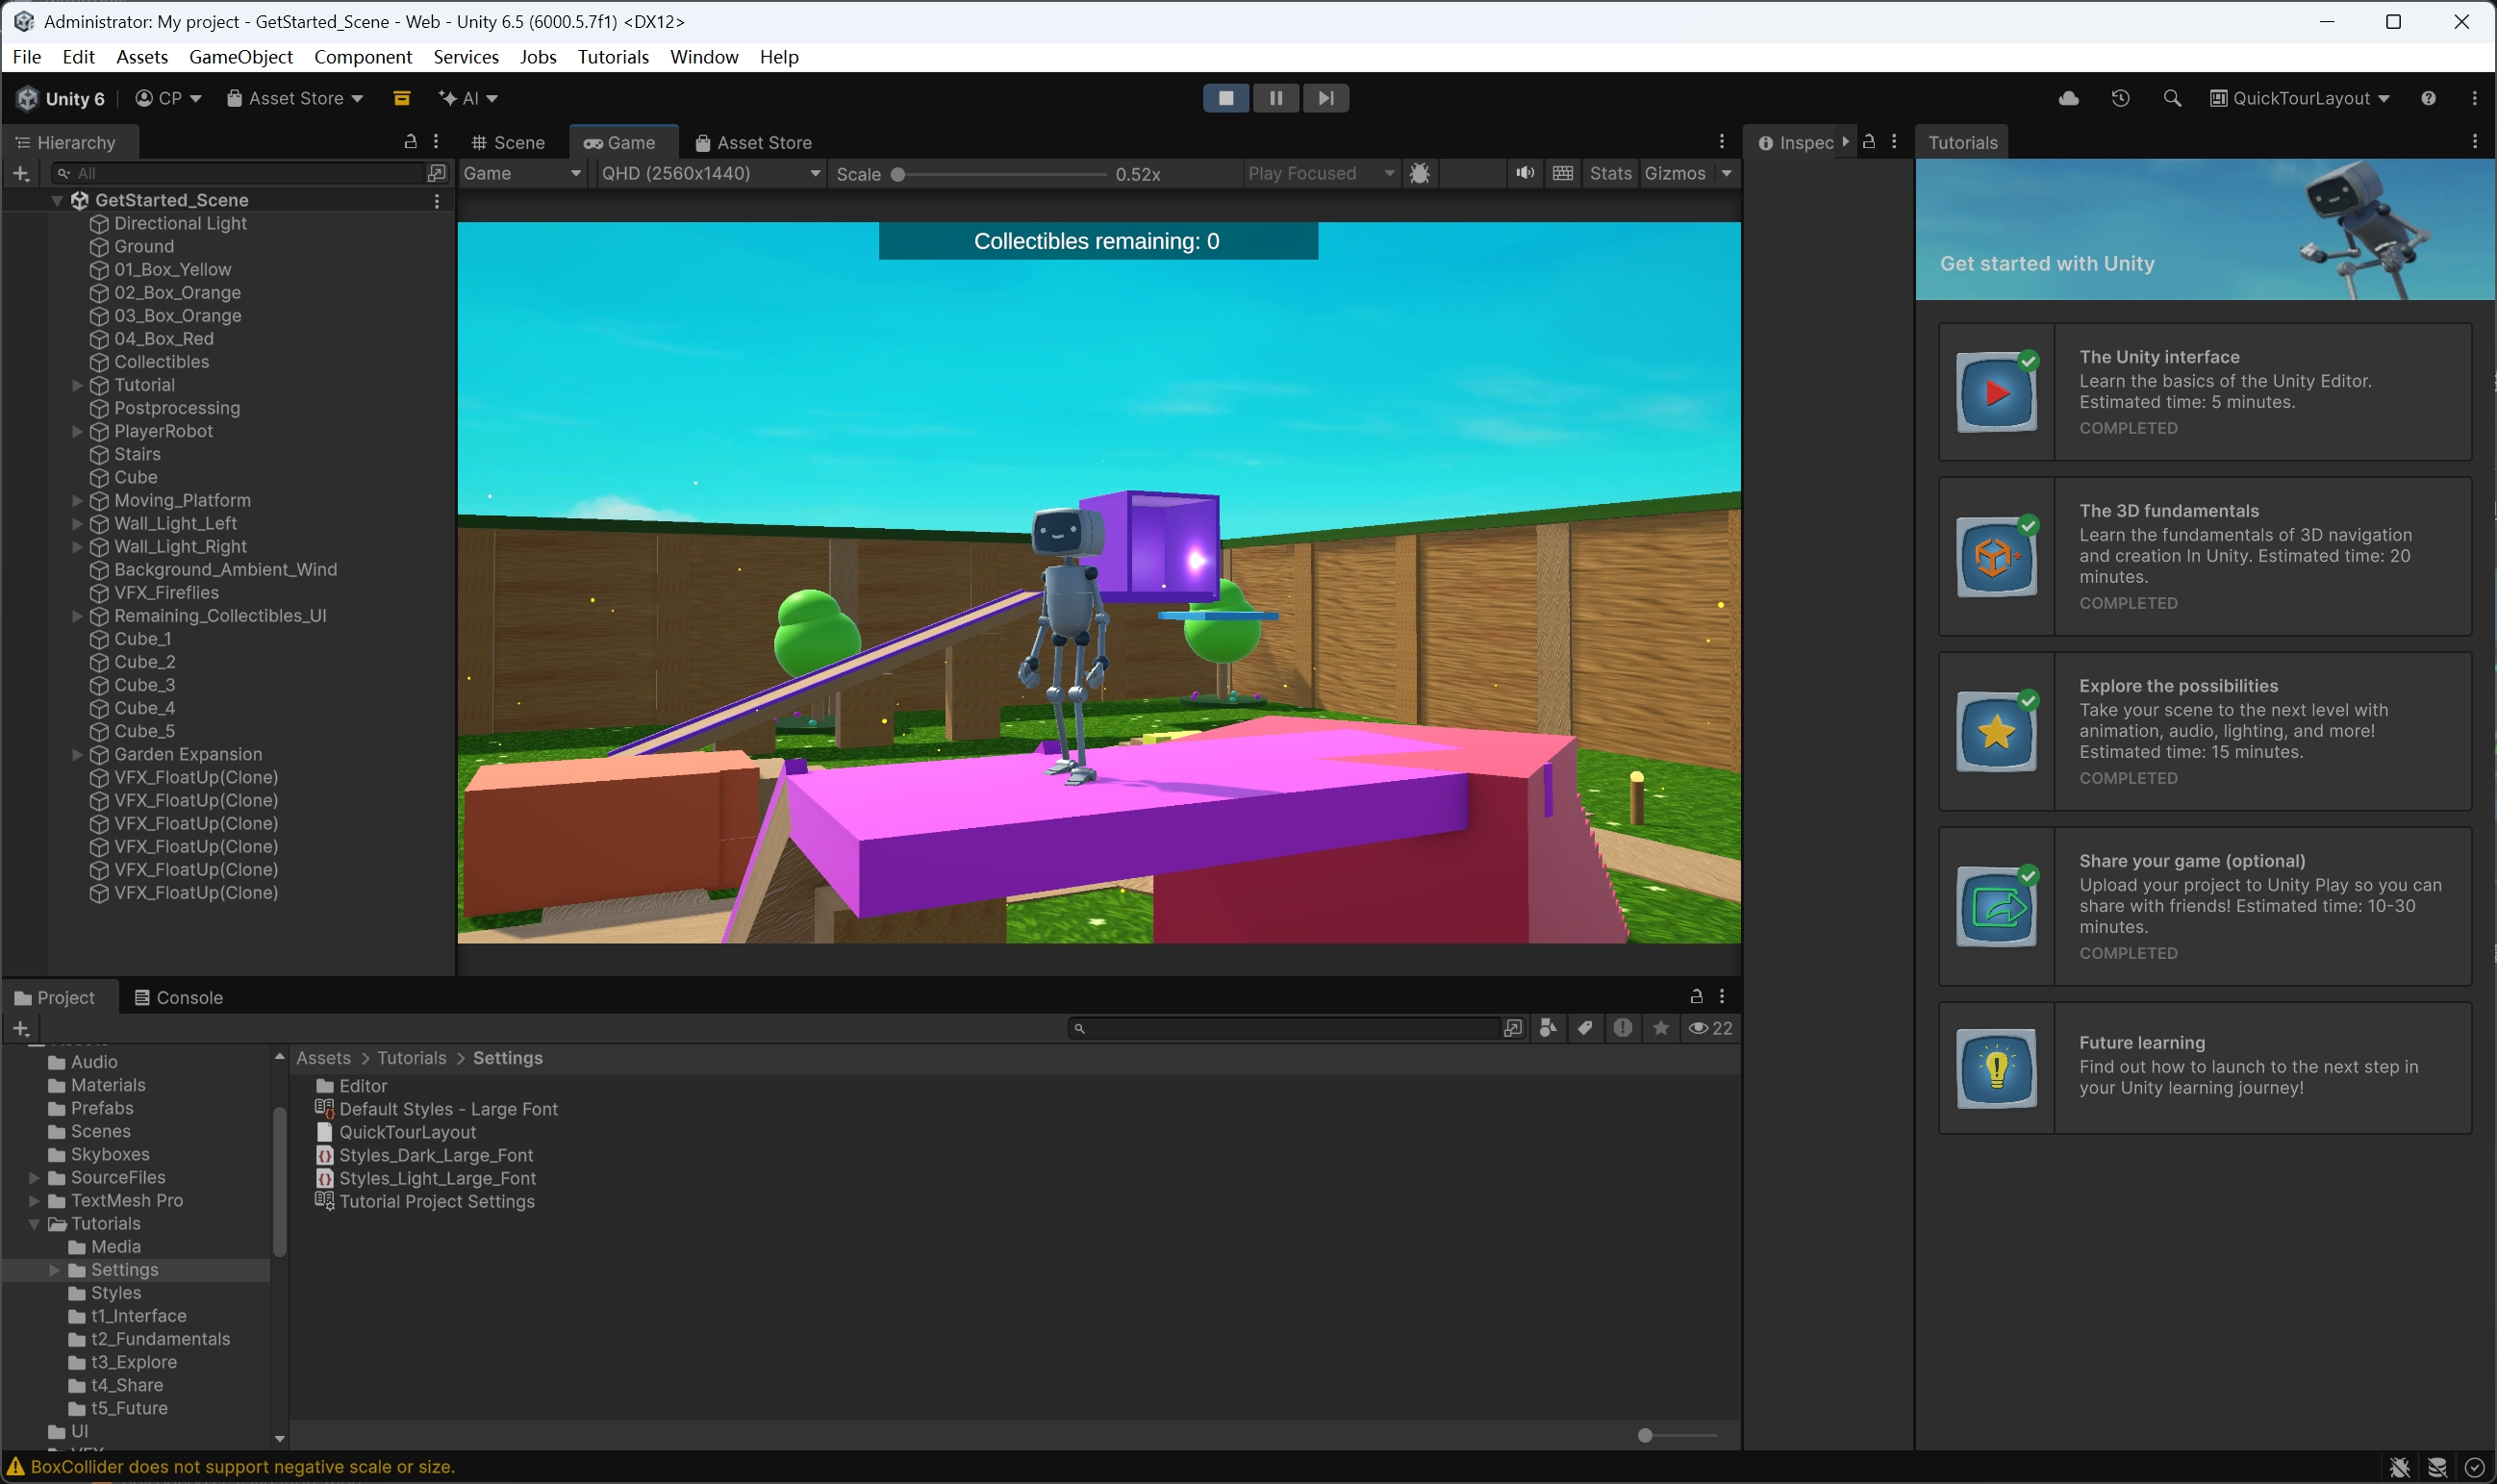
\includegraphics[width=\linewidth]{u7.jpg}
        \small (b) Elevated platform and ramp
    \end{minipage}

    \vspace{0.6em}
    \begin{minipage}[t]{0.49\textwidth}
        \centering
        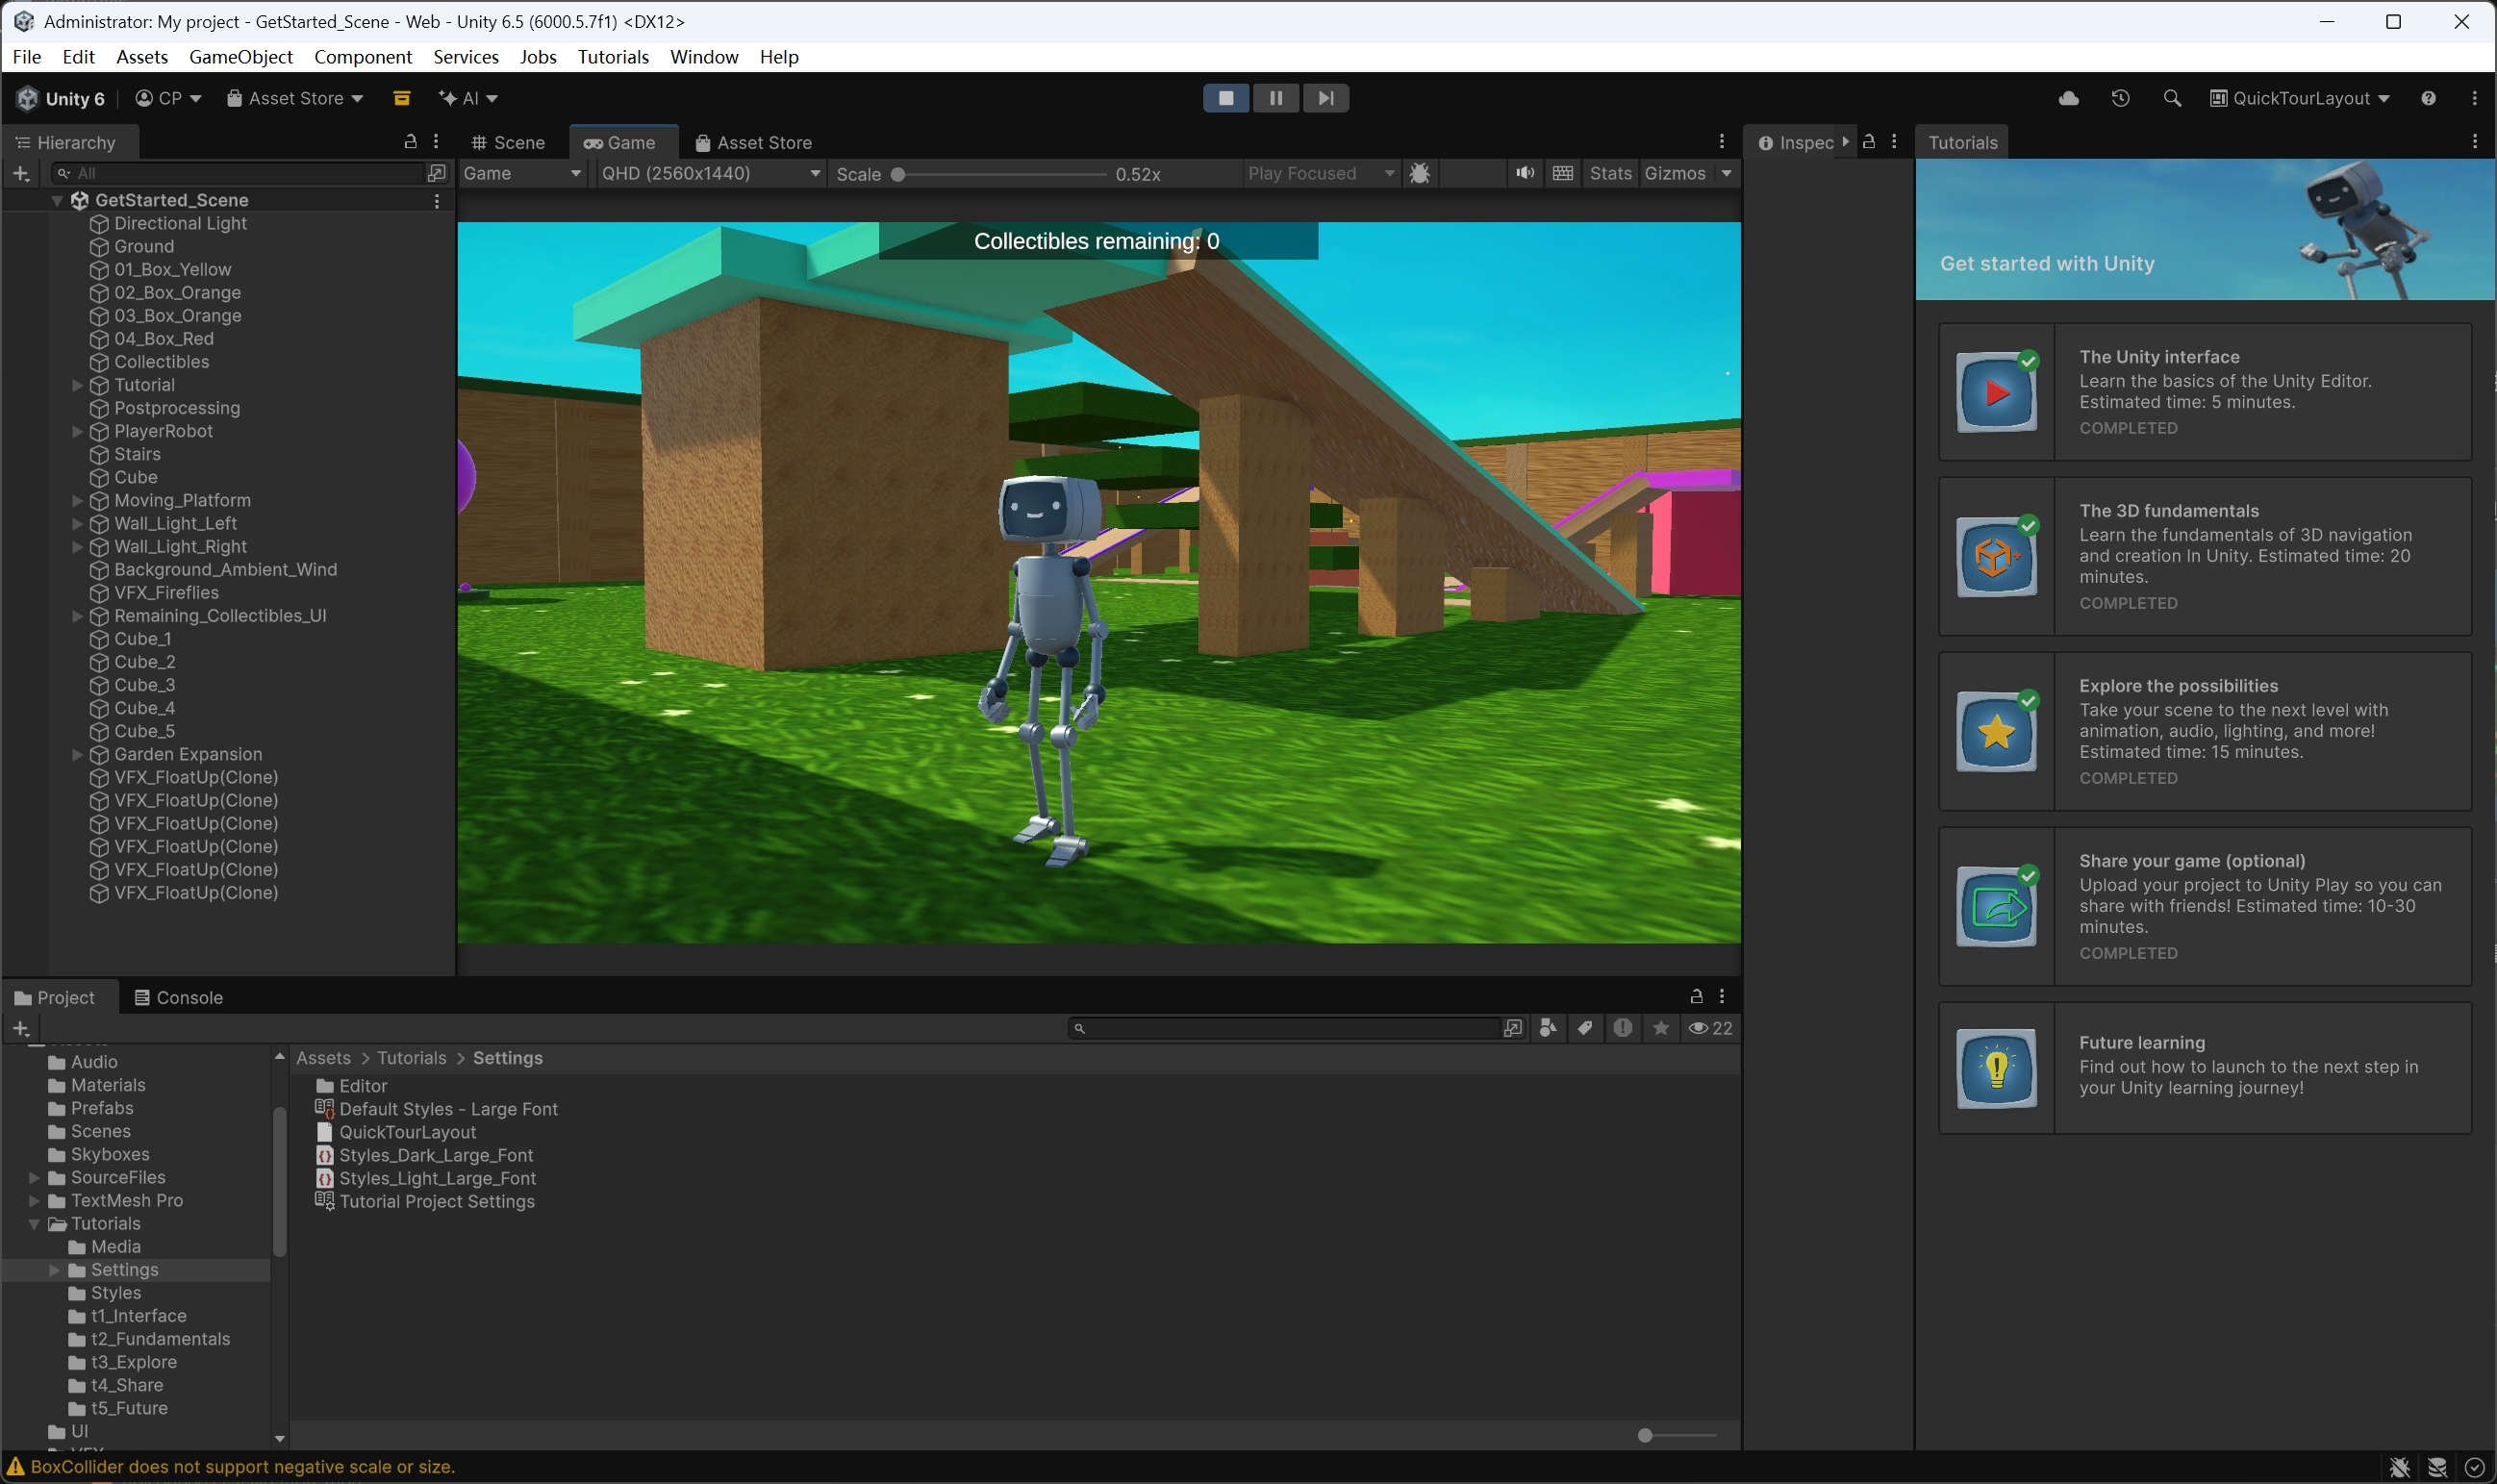
\includegraphics[width=\linewidth]{u8.jpg}
        \small (c) Supporting structures below the ramps
    \end{minipage}\hfill
    \begin{minipage}[t]{0.49\textwidth}
        \centering
        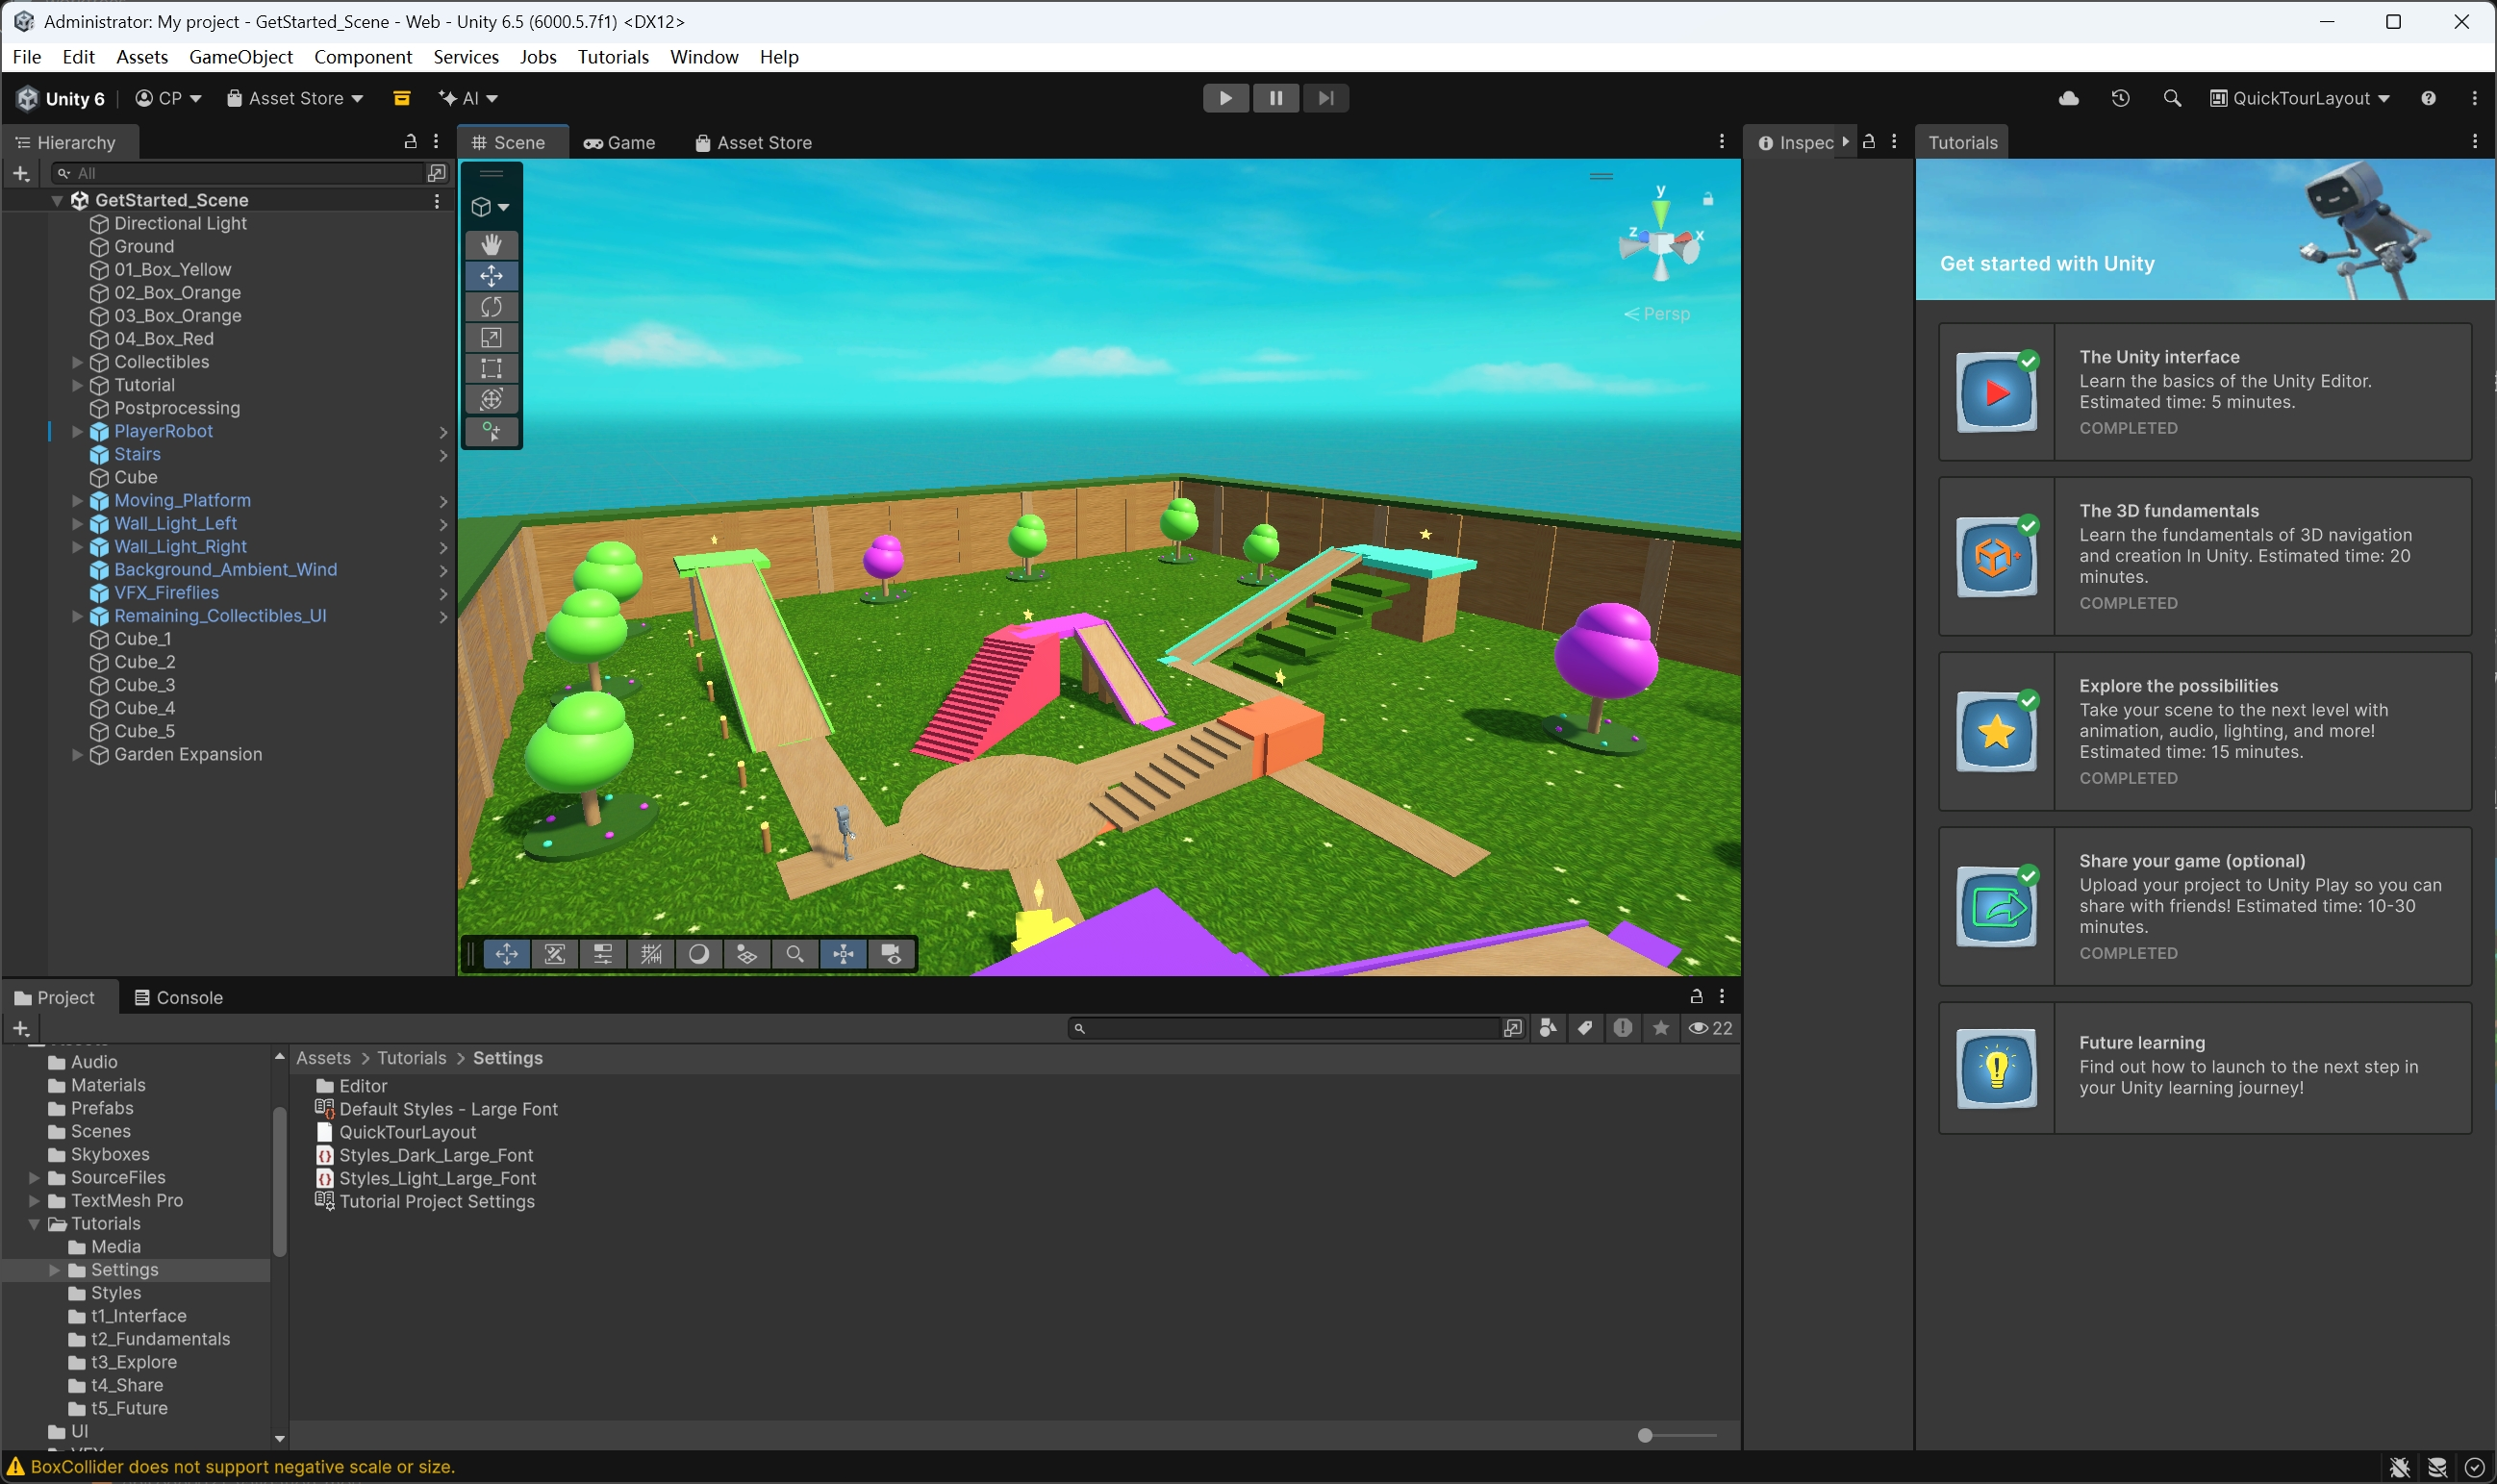
\includegraphics[width=\linewidth]{u9.jpg}
        \small (d) Overview of the expanded garden scene
    \end{minipage}
    \caption{Four views of the extended robot scene.}
\end{figure}


\end{document}
